\documentclass[headsepline,titlepage,ngerman,twoside,12pt]{report}
\usepackage[utf8]{inputenc}
\usepackage[T1]{fontenc}
\usepackage{lmodern}
\usepackage[ngerman]{babel}
\usepackage[a4paper,top=4cm,bottom=3cm,left=4cm,right=3cm]{geometry}
\usepackage[pdftex]{graphicx}
\usepackage{setspace}
\usepackage{csquotes}
\usepackage{tabularx}
\usepackage{xcolor}
\usepackage{listings}
\usepackage{booktabs}
\usepackage{amsmath}
\usepackage{comment}
\usepackage{aurl}
\usepackage{microtype}
\usepackage{xcolor}
\usepackage{natbib}
\usepackage{hyperref}
\usepackage{acronym}
\usepackage{multicol}
\usepackage{cleveref}
\usepackage{epigraph}
\PassOptionsToPackage{pdfborder={0 0 0}}{hyperref} %Für finale gedruckte Ausgabe, ohne hervorgehobene Links
%\usepackage{hypernat}
\daurl{ob}{http://www.snik.eu/ontology/ob/}
\daurl{bb}{http://www.snik.eu/ontology/bb/}
\daurl{ciox}{http://www.snik.eu/ontology/ciox/}
\daurl{he}{http://www.snik.eu/ontology/he/}
\daurl{it4it}{http://www.snik.eu/ontology/it4it/}
\daurl{meta}{http://www.snik.eu/ontology/meta/}
\author{Max Niclas Wächtler}
\newcommand\idea[1]{\textcolor{red}{#1}}

\newcommand\todo[1]{TODO: \textcolor{teal}{#1}}
%show comments for students, comment out for finished work or remove the todo statements and their content
%\newcommand\todo[1]{}%hide comments for students, uncomment for the finished work 
%remove "Kapitel X" headers *****
\setlength{\parindent}{0em}

\begin{document}
\allowdisplaybreaks%Mathe darf auch umbrechen
\lstset{language=SQL,morekeywords={PREFIX,owl,createElement,rdf,rdfs,meta,FILTER,str,bb,ob,SAMPLE,STR,AS,REPLACE,LANGMATCHES,skos,LANG,LIMIT}}

\onehalfspace

\begin{titlepage}
\thispagestyle{empty}
\begin{center}

{\large\bf UNIVERSITÄT LEIPZIG\\[1mm]}
Institut für Medizinische Informatik, Statistik und Epidemiologie (IMISE)

\vspace*{4cm}

{\Huge\textbf{Automatische Erstellung von Quizfragen aus einer Ontologie von Krankenhausinformationssystemen}\\}
\vspace{0.5cm}
{\large Besondere Lernleistung}\\
\vspace{2cm}

\vspace*{4cm}

\begin{tabularx}{\textwidth}{Xr}
Leipzig, Dezember 2020		&vorgelegt von:\\
\\
				&Max Niclas Wächtler\\
				&geb. am: 17.05.2003\\
\\
				&Betreuer:\\
				&Konrad Höffner\\
\end{tabularx}
\vspace{1cm}

\end{center}
\end{titlepage}
\newpage
\begin{abstract}
%Kurzreferat von Januar
Krankenhausinformationssysteme sind Informationssysteme, die sich in medizinischen Umgebungen mit der Verarbeitung von Daten, Informationen und Wissen beschäftigen.
Informationssysteme bestehen aus Hardware, Software als auch Anwendern. Kompetenz in der Nutzung von Krankenhausinformationssystemen ist wichtig, um in Krankenhäusern beispielsweise die Zusammenarbeit mit Patienten effektiv und zeitsparend zu gestalten.
Jedoch müssen Anwender diese Kompetenz erst einmal durch Quellen wie Lehrbücher erwerben, welche jedoch verschiedene Sichten auf das Themengebiet aufweisen und keinen schnellen Überblick über bestimmte Themen bieten können. Um dieses Problem anzugehen, habe ich mir als Ziel dieser besonderen Lernleistung gesetzt, ein Programm zu entwickeln, welches diese Informationen aus einer Ontologie, also eine Menge von Begrifflichkeiten mit Beziehungen untereinander, über eine Schnittstelle entnimmt, diese nutzerfreundlich in Form von zufällig generierten Fragen aufarbeitet und dem Nutzer ausgibt. Diese sollen eine grammatikalisch korrekte Form aufweisen und nebst der richtigen Antwort auch falsche Antworten enthalten, die trotzdem logisch wirken sollen, anstatt ein Zufallsverfahren zur Auswahl zu nutzen. 
\end{abstract}
\tableofcontents
\newpage


\section*{Begriffs- und Abkürzungsverzeichnis}
\begin{acronym} [SPARQL]
\acro{SPARQL}{SPARQL Protocol and RDF Query Language}
\acro{W3C}{World Wide Web Consortium}
\acro{KI}{Künstliche Intelligenz}
\acro{RDF}{Resource Description Framework}
\acro{HTML}{Hypertext Markup Language}
\acro{XML}{Extensible Markup Language}
\acro{URIs}{Universal Resource Identifier}
\acro{SNIK}{Semantisches Netz des Informationsmanagements im Krankenhaus}
\acro{WWW}{World Wide Web}
\acro{W3C}{World Wide Web Consortium}
\acro{HTTP}{Hypertext Transfer Protocol}
\acro{MIG}{Management von Informationssystemen im Gesundheitswesen}
\end{acronym}

\chapter{Einleitung}
\label{ch:Einleitung}
\section{Gegenstand und Motivation}
\label{sec:gegenstand}
\subsection{Gegenstand}
\label{sub:Gegenstand}
Das \ac{SNIK} ist ein abgeschlossenes Projekt, welches Begriffe des Informationsmanagements in dem Teilgebiet der medizinischen Informatik sowie deren Beziehungen untereinander beschreibt.
Es ist in der Lage, dieses Wissen in einer Ontologie darzustellen und diese sowohl maschinen- als auch menschenlesbar auszugeben.
Dabei nutzt es ein dem Semantic Web Stack ähnliches Modell (\cref{img:semanticwebstack2}), welches Anwendungen wie dem \ac{SNIK} Graph ermöglicht, Informationen abzufragen und diese Endnutzern in aufbereiteter Form zur Verfügung zu stellen.
\begin{figure}
\centering
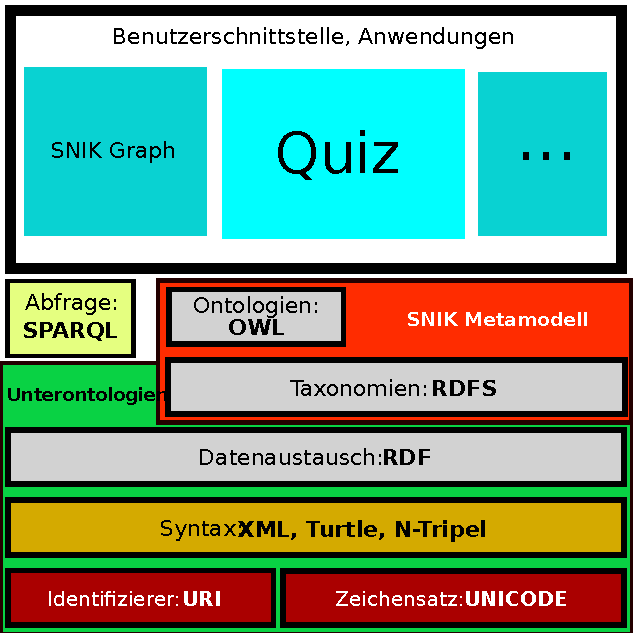
\includegraphics[width=0.7\textwidth]{images/swebstackde_snik.pdf}
\caption{Das semantische Modell von SNIK.}
\label{img:semanticwebstack2}
\end{figure}
Das Projekt konzentriert sich hauptsächlich auf Wissen der medizinischen Lehre. Dieses wird für Krankenhausinformationssysteme zur Verfügung gestellt, um die Arbeit für medizinisches Personal zu erleichtern. Speziell hat der durch Prof. Dr. Alfred Winter geleitete Teilbereich \ac{MIG} die Zielsetzung, durch Entwicklung von Methoden und Werkzeugen für das Informationsmanagement zu einer besseren Gesundheitsversorgung beizutragen.

Um nicht mit Ontologien versierten Nutzern eine Anwendung, die die Daten des Projektes nutzt, darzustellen, wurde unter anderem auch ein einfaches Multiple-Choice-Quiz auf Basis eines öffentlich verfügbaren Templates programmiert.
Diese nutzt die Ontologie hinter SNIK, um Anwendern einfache, automatisch generierte Fragen zu stellen.
Diese Fragen werden mithilfe der typisierten, gerichteten Verbindungen zwischen einzelnen Begriffen erzeugt, wobei das Quiz aus der SNIK-Ontologie zwei Gruppen von Verbindungen nutzt:
\begin{itemize}
    \item 1. Objekt A definiert Objekt B (A defines B),
    \item 2. Objekt A beschreibt die Verbindung zweier Objekte B und C (B is related to C in way A)
\end{itemize}
Dadurch werden für jeden Verbindungstyp unterschiedliche Fragen generiert.
Für Definitionen generiert sich der Fragetitel hierbei zum Beispiel nach dem folgenden Muster:
\newline \enquote{What is defined by A?}\newline
Unabhängig vom Fragetyp werden jeder Frage noch verschiedene Antworten zugeteilt.
Dazu zählt einmal die richtige Antwort, neben der aber auch drei andere, falsche Antworten durch einfache SPARQL-Queries generiert werden. 

\todo{
\begin{itemize}
\item In welcher Welt/Domäne oder welchem Arbeitsbereich/-gebiet bewegen wir uns im Rahmen der Seminararbeit/der ausgewählten Papers?
\item Worum geht es eigentlich?
\end{itemize}
Aus den Papers bzw. dem Antrag des Forschungsprojektes entnehmen.
}

\subsection{Problematik}
\label{sub:Problematik}
\todo{generell im gesamten text: jeden satz auf eine zeile}
Die Nutzer sollen möglichst mit logischen, aber nicht zu einfachen Fragen herausgefordert werden.
Um mithilfe des Multiple-Choice-Quiz ihren Wissensstand zu verbessern, sollte das Quizprogramm bestimmte Vorgaben erfüllen und diese auch in der Qualität der Fragen widerspiegeln.
Das stellt sich als relativ schwer heraus, da die Implementierung von natürlichsprachlicher Grammatik sich seit jeher als ein Problem in der Informatik herausstellt.
\paragraph{Korrektheit}
\label{para:Korrektheit}
Für den Anwender soll die Frage gut lesbar und in seiner Grammatik verständlich sein.
Da die Quizfragen in einem bestimmten Zeitfenster bearbeitet werden sollen, ist es wichtig, dass sie schnell vom Nutzer verstanden werden.
Da der Hauptzweck die Selbstüberprüfung ist, werden dadurch fehlende Korrektheit gegenüber dem User die Ergebnisse verfälscht , was zu einer falschen Selbsteinschätzung führt.
\paragraph{Übersichtlichkeit}
Eine Frage muss für den Nutzer übersichtlich gestaltet sein.
Sie soll schnell durchgelesen sein, damit er den metaphorischen \enquote{Faden} nicht verliert und Fragen nicht erneut lesen muss.
Um dies zu garantieren, muss die Anzahl der Zeichen im Fragetitel eine bestimmte Zahl nicht übersteigen.
Dies kann zum Beispiel bei langen Definitionen (Fragetyp 1) ein Problem sein.
\paragraph{Qualität}
Neben den anderen beiden Bedingungen muss bei Fragen auch die Qualität und das Niveau der Frage sowie des Quiz allgemein hoch gehalten werden.
Doch das ist im bereits existenten Quiz an vielen Stellen nur teilweise vorhanden, was sich in verschiedenen Aspekten widerspiegelt.
Darunter fallen zum Beispiel die Erwähnung der richtigen Antwort im Fragetitel bei z.B. Definitionen oder in einfacheren Punken wie z.B. dem Doppeln von Fragen.
Dadurch wird der Nutzer nicht genug herausgefordert, was dazu führt, dass er die Fragen nicht mithilfe seines Fachwissens, sondern einfach durch logisches Denken beantworten kann. 
\paragraph{Heterogenität}
Das Quiz sollte für den Nutzer möglichst einen großen Teil der Möglichkeiten der SNIK-Ontologie anschaulich machen.
Da jedoch das existierende Quiz nur zwei der 18 Typen von Verbindungen zwischen Objekten nutzt, die in der SNIK-Ontologie vorkommen, variieren die Fragetypen nur wenig, was auf Dauer für Nutzer langweilig oder anstrengend wird. Außerdem wird dadurch ein großer Teil des verfügbaren Wissens nicht abgefragt, 
\\\\\todo{
\begin{itemize}
\item Worin bestehen die Probleme?
\item Warum ist die geschilderte vorliegende Situation problematisch?
\item Für wen ist sie problematisch?
\end{itemize}
Aus den Papers bzw. dem Antrag des Forschungsprojektes entnehmen.\\
}\todo{
Hier ist auf die generelle Problemlage einzugehen, die dem Aufsatz im Wissenschaftsfeld zu Grunde liegt.\\
Bsp.: Daten aus der Krankenversorgung stehen aus rechtlichen und technischen Gründen nicht für die Forschung zur Verfügung, sodass klinische Forscher eigene Datenerhebungen planen müssen.
}
%erfüllt soweit, evtl noch bissl Formulierung (TP)
\subsection{Motivation}
\label{sub:Motivation}
%snik.eu nehmen
Das Ziel des SNIK-Projektes ist es, ein theoretisch und empirisch begründetes, sowie erprobtes Semantisches Netz des Informationsmanagements im Krankenhaus (SNIK), das die Konzepte des Informationsmanagements beschreibt und verbindet, zu kreieren.
Um Medizinstudenten und anderen Mitarbeitern aus dem medizinischen Umfeld eine beispielhafte Nutzungsmöglichkeit für diese Ontologie zu bieten und ihnen einen einfachen Zugriff neben dem SNIK-Graph auf das Themengebiet zu ermöglichen, kann ein Multiple-Choice-Quiz einen einfachen Einblick auf die Einsatzmöglichkeiten von einer Ontologie aus Krankenhaussystemen bereitstellen und Interessenten aus nichtinformatischen Teilgebieten eine Vorstellung ermöglichen.

\todo{
\begin{itemize}
\item Warum lohnt es sich, die genannten Probleme zu lösen?
\item Wer wird welchen Nutzen von dieser Abschlussarbeit haben?
\item Warum sind die Papers wichtig?
\end{itemize}
Aus den Papers bzw. dem Antrag des Forschungsprojektes entnehmen.
}
\todo{
Worin liegt der zusätzliche Nutzen, die beiden Ansätze zu vergleichen? Worin liegt der Nutzen, den Ansatz des Papers auf die Problematik des Forschungsprojektes anzuwenden?\\
Bsp.: Gelänge es, Daten aus der Krankenversorgung vollständig zu anonymisieren, könnten sie für beliebige Forschungsvorhaben genutzt werden.
}

\section{Zielsetzung}
\label{sec:Ziele}
Das Ziel meiner besonderen Lernleistung ist es, automatisch Multiple-Choice-Quizfragen auf Basis der SNIK-Ontologie zu generieren. 
Dazu wird ein existierender Prototyp analysiert und hinsichtlich der oben genannten Qualitätsmaße optimiert.
\begin{itemize}
\item Ziel Z1: Analysieren des vorhandenen Prototyps
\item Ziel Z2: Optimieren des vorhandenen Prototyps
\end{itemize}

\section{Vorgehensweise}
\label{sec:Vorgehen}
\todo{
Stellen Sie Ihre Methode bzw. Herangehensweise dar.
Was ist Ihre konkrete Aufgabenstellung im Rahmen der Seminararbeit? Das könnte z.B. sein:
\begin{itemize}
\item Vorstellen verschiedener Lösungsansätze, Vergleich und Bewertung der Lösungsansätze, Literaturrecherche nach weiteren vergleichbaren Papers.
\item Bewertung eines Lösungsansatzes hinsichtlich einer konkreten Forschungssituation.
Literaturrecherche nach weiteren vergleichbaren Papers.
\end{itemize}
}

\todo{
Beschreiben Sie Ihre Vorgehensweise in einzelnen Schritten und stellen Sie die Reihenfolge der Abarbeitung dar.
Auf diese Punkte sollten Sie in der Diskussion wieder eingehen.
}
\todo{
\begin{enumerate}
\item Schritt 
\item Schritt 
\end{enumerate}
}
\todo{
Vermeiden Sie Formulierungen wie \enquote{Es ist nicht bekannt, ob...} oder \enquote{Es existiert kein...}.
Solche Formulierungen kehren in der Regel einfach das bereits angedachte Lösungsmodell um und postulieren das Fehlen der angedachten Lösung einfach als Problem.
... \\
Schritt n\\
Das ist ähnlich, wie wenn es in der Werbung hieße \enquote{Wenn Sie das Problem haben, dass Ihnen Aspirin fehlt, dann kaufen Sie doch Aspirin.}
Sinnvoller ist diese Aussage: \enquote{Wenn Sie das Problem haben, dass Ihnen der Kopf weh tut, dann kaufen Sie doch Aspirin.}
Es ist also bei der Problembeschreibung erforderlich, sich in die Lage dessen zu versetzen, den man mit der angedachten Lösung beglücken möchte.
Sein Problem ist zu ermitteln und so zu formulieren, er/sie das Problem wiedererkennt und dadurch geneigt ist, sich für die Lösung des Problems zu interessieren.
} 
\begin{itemize}
    \item Aufgabe A1.1 zu Ziel Z1: Analyse der Strategien zur Generierung der Stämme und Distraktoren
    \item Aufgabe A2.1 zu Ziel Z2: Entwickeln neuer Strategien zur Generierung der Stämme
    \item Aufgabe A2.2 zum Ziel Z2: Entwickeln neuer Strategien zur Generierung von Distraktoren
    \item Aufgabe A2.3 zum Ziel Z2: Aufstellen von Regeln zur Nutzerfreundlichkeit der Fragen
\end{itemize}

\todo{(2--3 Seiten)}
\chapter{Grundlagen}
\label{ch:Grundlagen}

\section{Semantic Web}
\label{sec:semanticweb}
Das Semantic Web (oder auch: semantisches Netz) stellt eine Methode dar, um maschinenlesbares Wissen über das \ac{WWW} in Form von HTML-Dokumenten zu verbreiten.
Anders als bei der klassischen Website aber wird hier nicht nur primär Wert auf die Lesbarkeit durch einen Menschen, sondern auch auf die Maschinenlesbarkeit Wert gelegt, indem die Seite nebst dem normalen HTML-Code auch Informationen, die durch Computer gelesen werden können, hinterlegt. Diese sind durch Technologien des semantischen Webs ( \acs{RDF}, \acs{SPARQL}, ... ) einles- und verarbeitbar. 

\subsection{\acs{WWW}}
\label{sub:www}
Das \ac{WWW} bildet ein verknüpftes Kommunikationsmodell zwischen allen Ressourcen und Nutzern des Internets, die das \ac{HTTP} nutzen.
Es wurde vom Direktor der \ac{W3C} Tim Berners-Lee 1991 entwickelt und ermöglicht den Zugriff auf sowie den Datenaustausch mit \acs{HTML}-Dokumenten.
Es definiert also das, was die Allgemeinheit als \enquote{das Web} bezeichnet.


\subsection{Linked Data}
\label{sub:linkeddata}
Der Begriff \enquote{Linked Data} bezieht sich auf eine Reihe bewährter Methoden zum Veröffentlichen und Verbinden strukturierter Daten im Web.
Es verknüpft Dateien aus dem semantischen Web untereinander, sodass sie durch semantische Abfragen benutzbar werden.
Linked Data basiert auf standardisierten Modellen für den Datenaustausch im Web, besipielsweise \acs{HTML}, um auch wie beim semantischen Prinzip maschinenlesbare Daten zu generieren.
Zielsetzung von Linked Data ist es, das Internet zu einer globalen, computerverbarbeitbaren Datenbank weiterzuentwickeln und so den Zugriff für technische Endgeräte weiter zu vereinfachen.

\subsection{\acs{RDF}}
\label{sub:rdf}
\ac{RDF} ist ein weiteres Standardmodell für den Datenaustausch im Web, welches in den 90er Jahren des letzten Jahrtausends seine Anfänge findet.
Im Gegensatz zu \ac{HTML} und \ac{XML} ist es in der Lage, enthaltene Informationen zu kombinieren und weiter zu verarbeiten, anstatt diese nur korrekt anzuzeigen.
Daher ist RDF auch oft als grundlegendes Repräsentationsformat für die Entwicklung im Semantic Web angesehen.
Es erweitert die Verknüpfungsstruktur von diesem, um \ac{URIs} einzubinden.
Solche URIs werden im semantischen Netz dazu genutzt, Beziehungen zwischen Dingen beziehungsweise zwischen den beiden Enden der Verknüpfung herzustellen, um Dateien zu verknüpfen, verfügbar zu machen und für Anwendungen freizugeben.
Dadurch können Daten zusammengeführt werden, die sich eigentlich im Schema grundlegend unterscheiden, ohne dass alle Datenkonsumenten geändert werden müssen.
Diese Zusammenführung geschieht in einem Schichtenmodell: Aussagen werden als Tripel modelliert und bilden eine Aussage, die aus Subjekt, Prädikat und Objekt zusammengefügt werden kann.
Man kann also einen Tripel mit einem einfachen Satz vergleichen: als Beispiel hier einmal der Teilsatz \textit{Google produziert Prozessoren}.
Hier stellt \textit{Google} das Subjekt dar, \textit{produziert} ist das Prädikat und \textit{Prozessoren} sind das Objekt.
Hat man eine Menge von Tripeln, bilden diese ein semantisches Netz, was tabellarisch übersichtlich dargestellt werden kann, siehe \cref{tab:rdfexample}.

\begin{table}
\begin{centering}
\begin{tabularx}{\textwidth}{XXX}
\toprule
\textrm{Subjekt}			&\textrm{Prädikat}			&\textrm{Objekt}\\
\midrule
New York				&liegt in				&USA\\
USA				 		&liegt in				&Nordamerika\\
Nordamerika				&liegt in				&Amerika\\
Südamerika				&liegt in 			&Amerika\\
\bottomrule
\end{tabularx}
\end{centering}
\caption{Beispiel für RDF-Tripel.}
\label{tab:rdfexample}
\end{table}


\subsection{\acs{SPARQL}}
\label{sub:sparql}
\ac{SPARQL} ist ein Standard für die Abfrage von in \ac{RDF} spezialisierten Informationen sowie für die Darstellung der zugehörigen Resultate, siehe \cref{img:semanticwebstack1}.
Es basiert auf einfachen \ac{RDF}-Anfragen in Form von Graphmustern, also einer Menge von Tripeln, enthält jedoch auch erweiterte Funktionen für die Konstruktion komplexerer Anfragemuster, die Verwendung zusätzlich hinzufügbarer Filterbedingungen und für die Formatierung der schlussendlichen Ausgabe.


Man kann also \ac{SPARQL} als eine faktische Abfragesprache des semantischen Webs bezeichnen.
\begin{figure}
\centering
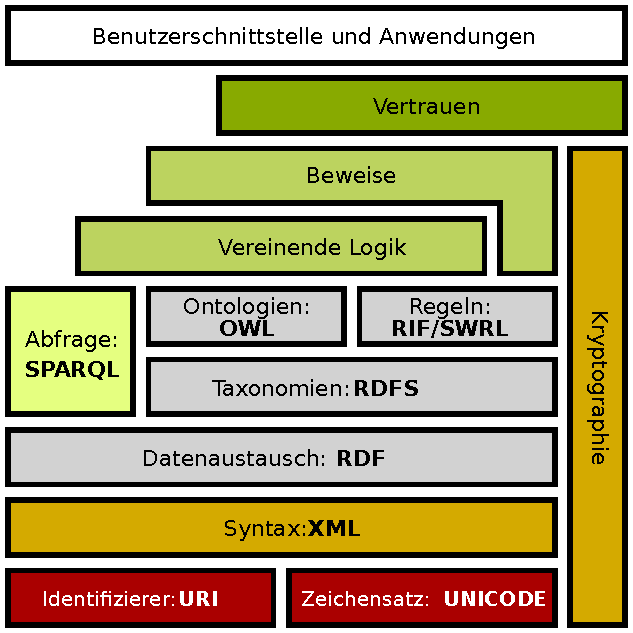
\includegraphics[width=0.7\textwidth]{images/swebstackde.pdf}
\caption{Der Semantic Web Stack.}
\label{img:semanticwebstack1}
\end{figure}

\subsection {Ontologien}
\label{sub:ontologien}
\setlength\epigraphwidth{.9\textwidth}
\setlength\epigraphrule{0pt}

\epigraph{\itshape An ontology is an explicit specification of a conceptualization.}{---Thomas R. Gruber\todo{quelle zitieren}}

\noindent Ontologien sind (im informatischen Kontext) meist sprachlich gefasste und geordnete Darstellungen einer Menge von Begrifflichkeiten mit festen Beziehungen untereinander.
Diese Beziehungen befassen sich stets auf einen bestimmten Gegenstandsbereich und werden dazu genutzt, Wissen in digitalisierter Form zwischen Anwendungen und Diensten auszutauschen.
Dabei müssen bestimmte Interferenz- und Integritätsregeln eingehalten werden, also Regeln zu Schlussfolgerungen sowie zu der Gewährleistung ihrer Gültigkeit.
Ontologien erfreuen sich seit der Idee des semantischen Webs einem stets wachsenden Bekanntheitsgrad, was dazu führt, dass sie als Teil der Wissensrepräsentation im Teilgebiet \acs{KI} einen großen Einfluss haben.
Dabei beschreibt die Idee des Semantic Web eine Erweiterung des vorhandenen Netzes, um Daten zwischen Rechnern einfacher austausch- und verwertbar zu machen und sie somit besser zu explizieren, anstatt sie unkonstruiert stehen zu lassen.
Zum Sinne dieser Realisierung dienen Standards zur Veröffentlichung und Nutzung maschinenlesbarer Daten -- insbesondere \ac{RDF}.

\subsection{Künstliche Intelligenz}
\label{sub:ki}

\ac{KI} ist ein Teilgebiet der Informatik, welches sich mit der Automatisierung intelligenten Verhaltens befasst.
Es spiegelt eine Möglichkeit wieder, bestimmte Entscheidungsstrukturen des Menschen nachzubilden und es somit Computern zu ermöglichen, komplexe Probleme selbstständig zu bearbeiten und zu lösen.
Um diese Informationen weiter zu nutzen, können Methoden des Semantic Web genutzt werden, um sie als Tripel einfach maschinenlesbar darzustellen und für andere Computer verfügbar zu machen.

\section{Informationssysteme}
\label{sec:informationssysteme}

Ein Informationssystem ist ein System, welches durch die Bildung logischer Zusammenhänge eine Deckung der Informationsnachfrage zur Aufgabe hat.
Es produziert, beschafft, verteilt und verarbeitet Daten durch eine Zusammenarbeit zwischen Mensch und Technik durch Aufgaben.

\subsection{Krankenhausinformationssystem}
\label{sub:kis}
Krankenhausinformationssysteme beschreiben die Gesamtheit aller Informationssysteme zur Produktion, Beschaffung, Verteilung und Verarbeitung von medizinischen und administrativen Daten im Krankenhaus.
Dazu gehören verschiedene Formen der Datenbereitstellung sowie auch konventionelle Methoden der papierbasierten Dokumentation und der sprachlichen Kommunikation.
Das grundsätzliche Ziel eines Krankenhausinformationssystems ist, die Kommunikation zwischen Mitarbeitern zu verbessern und den Ablauf in Krankenhäusern zu steuern, indem Mitarbeitern gezielt Zugriff auf für ihn relevantes Wissen aus der ihm zugeteilten Benutzerrolle gegeben wird, zum Beispiel über den gerade zu behandelnden Patienten.

\subsection{Grundbegriffe}
\label{sub:begriffe}
\paragraph{Information}
\label{parag:information}
Information ist die Kenntnis über bestimmte Sachverhalte oder Vorgänge, im engeren Sinne über einzelne, konkrete, benennbare Objekte der realen und der virtuellen Welt. 

\paragraph{Wissen}
\label{parag:wissen}
Wissen ist die Kenntnis über den in einem Fachgebiet zu gegebener Zeit gegebenen Konsens, vor allem bezogen auf eine gültige Terminologie, erlaubte Interpretationen, bestehender Zusammenhänge und Gesetzmäßigkeiten sowie empfehlenswerter Methoden und Handlungen.
Wissen ist also auch Information, aber in dem Fall nicht auf einzelne Objekte, sondern eine Menge von Objekten und deren Beziehungen untereinander bezogen, vgl. \citet{his}.

\paragraph{Daten}
\label{parag:daten}
Daten sind Gebilde aus Zeichen oder kontinuierliche Funktionen, die durch bekannte oder unterstellte Beziehungen Informationen darstellen können.
Sie stellen die Grundlage oder das Ergebnis eines Verarbeitungsschrittes dar. 

\section{\acs{SNIK}-Projekt}
\label{sek:snik}
Das \ac{SNIK} ist ein vollendetes Projekt, welches Begriffe des Informationsmanagements sowie deren Beziehungen untereinander beschreibt.
Es ist in der Lage, diese Menge an Informationen in einer Ontologie darzustellen und diese sowie maschinen- als auch menschenlesbar auszugeben.
 Dabei nutzt es ein dem Semantic Web Stack ähniches Modell(\cref{img:semanticwebstack2}), welches Anwendungen wie dem \ac{SNIK} Graph oder einem Multiple-Choice-Quiz ermöglicht, Informationen abzufragen und diese Endnutzern in aufbereiteter Form zur Verfügung zu stellen.
Dabei konzentriert sich das SNIK-Projekt hauptsächlich auf die Daten der medizinischen Lehre, um diese für Krankenhausinformationssysteme zur Verfügung zu stellen und die Arbeit für medizinisches Personal zu erleichtern.
\begin{figure}
\centering
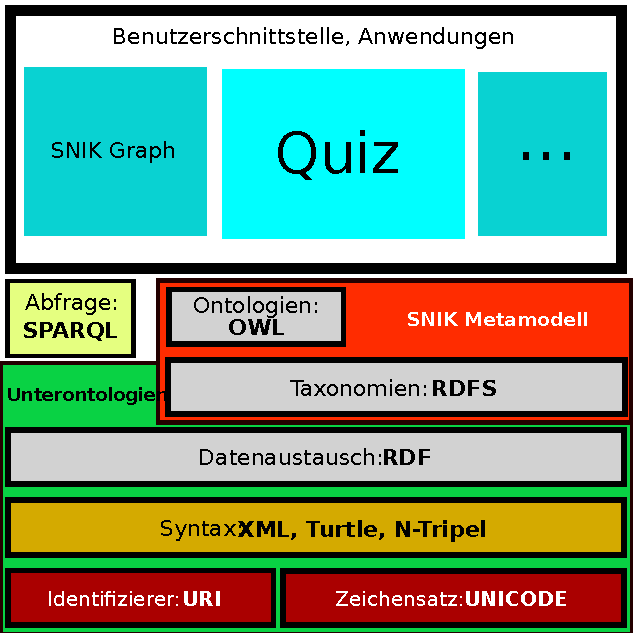
\includegraphics[width=0.7\textwidth]{images/swebstackde_snik.pdf}
\caption{Das semantische Modell von SNIK.}
\label{img:semanticwebstack2}
\end{figure}

\subsection{JavaScript}
\label{sub:js}
%\cite{fard2013jsnose}
JavaScript ist eine leistungsstarke und flexible Skriptsprache, die von Entwicklern zunehmend zur Erstellung interaktiver Webanwendungen eingesetzt wird.
Die Sprache ist dynamisch, schwach typisiert und verfügt über eine Vielzahl an für Webanwendungen essentiellen Funktionen. 
Sie lässt sich außerdem hervorragend mit anderen Websprachen wie CSS und HTML implementieren und besitzt die Fähigkeit, mit diesen zu interagieren.\\
JavaScript wird bei der Quiz-Webanwendung des SNIK-Projekts genutzt, um Fragen und Antworten anzuzeigen und diese dem Nutzer interaktiv zum Beantworten bereitzustellen.

\section{Multiple-Choice-Quiz}
\label{sec:quiz}
%Definition Multiple-Choice-Quiz aus DBpedia Clover Quiz, übersetzt aus dem Englischen, mit vgl
%\enquote{A multiple choice question consists of a stem (the question), a key (the correct answer) and distractors (a set of incorrect, yet plausible, answers).}\\
Ein Multiple-Choice-Quiz ist eine Ansammlung an Fragen, die allesamt aus einem Stamm (der Frage), einem Schlüssel (der richtigen Antwort) und mehreren Distraktoren (eine Menge von inkorrekten, aber plausibel klingenden Antwortmöglichkeiten), vgl. \todo{Quelle mit citet zitieren}
\\Ein Beispiel für eine solche Frage wäre hier aufgeführt:
\\\textit{Q: In einer Hand halte ich ein rotes, ein grünes und ein blaues Blatt Papier. Ich lege nun das rote und das blaue Blatt aus meiner Hand. Welche Farbe hat das Blatt, welches sich immer noch in meiner Hand befindet?}
\label{tab:quizexample}
\begin{itemize}
  \item Rot
  \item Grün
  \item Blau
\end{itemize}
Hierbei ist die Antwort \enquote{Grün} der Schlüssel. \enquote{Rot} und \enquote{Blau} sind \textit{Distraktoren}, die von dem Schlüssel ablenken sollen.
\\Der Sinn bei einem Multiple-Choice-Quiz besteht darin, den Befragten für richtige Antworten mit Punkten zu belohnen. Antwortet er falsch, bleibt seine Punktzahl entweder gleich oder Punkte werden abgezogen. Die Anzahl der vergebenen Punkte kann dabei von unterschiedlichen Faktoren abhängig gemacht werden, beispielsweise an der Zeit, die zum Lösen der Frage benötigt wurde.
\subsection{Distraktoren}
\label{sub:distraktoren}
Distraktoren beschreiben im Kontext eines Quiz falsche Antwortmöglichkeiten, die den Befragten von der richtigen Antwort ablenken sollen.
Durch sie soll vermieden werden, dass falschen Antworten durch Logik einfach von der richtigen Antwort unterschieden werden können. Der Sinn von Distraktoren ist es also, für den Befragten plausibel zu erscheinen.
Daraus resultierend kann eine schlechte Auswahl von Distraktoren Fragen um einiges einfacher gestalten. Nehmen wir dazu einmal als Beispiel unsere Frage im \cref{tab:quizexample}:
die Distraktoren klingen plausibel, da sie im Stamm der Frage erwähnt werden. Würde man hier allerdings andere Farben zur Auswahl stellen, die nicht im Kontext der Frage stehen und somit direkt ausgeschlossen werden können, zum Beispiel \enquote{Gelb}, könnte der Befragte diese logisch ausschließen. 

\chapter{Lösungsansatz}
\label{ch:Lösungsansatz}
\todo{Der Lösungsansatz ist eine kurze Beschreibung der Arbeitshypothese sowie des Vorgehens zur Lösung der in der Einleitung beschriebenen Probleme.}
Dieses Kapitel soll dazu dienen, den Lösungsweg der genannten Probleme genauer zu beschreiben.
Eine Erläuterung der Ausführung dieser erfolgt im nächsten Kapitel. 

\section{Lösungsansatz zu Aufgabe A1.1}
Um den bestehenden Prototyp zu verstehen und diesen zu erweitern bzw. zu verbessern, müssen wir dazu die Methodik zur Generierung der Fragen analysieren.
Diese Generierung hat die Zielsetzung, menschenlesbare Quizfragen zu erzeugen.
Dazu wird als Erstes im existierenden Prototyp eine Abfrage an die Ontologie gesendet, um die nötigen Daten für die Generierung der Frage zu erhalten.
Solche Abfragen werden in der SNIK-Ontologie durch SPARQL-Queries (\cref{sub:sparql}) gehandhabt. Gesendete Queries werden von einem Endpunkt auf dem SNIK-Server angenommen, welcher diese dann als Abfrage an die Ontologie weiterleitet und diese umsetzt. Diese Rückgabewerte werden dann in dem Quiz genutzt und mithilfe von einfachem JavaScript-Code im Browser des Benutzers in einfacher Wortform angezeigt. Um Ressourcen zu schonen, wird jedoch nicht bei jedem Aufruf des Quizzes eine einzelne Frage generiert - das Quiz greift auf eine große Liste aus vorher generierten Fragen zu.
Diese sind im JavaScript-Code, welcher durch den Browser angezeigt wird, fest implementiert.\\
\begin{comment}wie in diesem Beispiel deutlich wird:
\begin{lstlisting}
question: s.default.createElement("span", null, "Frage"),
answers: [
  s.default.createElement("span", null, "Antwort"),
  s.default.createElement("span", null, "Distraktor_1"),
  s.default.createElement("span", null, "Distraktor_2"),
  s.default.createElement("span", null, "Distraktor_3")
],
correct: 0
\end{lstlisting}
Für die Frage und die jeweiligen Antworten werden bei dem Quellcodeausschnitt jeweils eigene Elemente erstellt. Die Frage steht hierbei im Überelement question, während die Antwortmöglichkeiten im Überelement answers stehen. 
\end{comment}
Um den Inhalt dieser Fragen zu erhalten, muss eine Abfrage an den SPARQL-Endpunkt gesendet werden, der auf die Ontologie zugreift und mithilfe der Abfrage bestimmte Informationen an das Programm ausgibt.
Die erhaltenen Daten werden nun von dem Programm spezifisch für den Verbindungstyp verarbeitet, wie in \cref{sub:Gegenstand} schon erkärt wurde. Bei der spezifischen Verarbeitung gibt es eine wichtige Unterscheidung: die Methodik der Generierung des Stammes und die Methodik der Generierung der Distraktoren. Während ersteres für jeden Fragetyp unterschiedlich ist, werden Distraktoren stets gleich generiert. Hierzu müssen also im nächsten Abschnitt die Generierung der verschiedenen Fragen und Antworten analysiert werden.
\section{Lösungsansatz zu Aufgabe A2.1}
Um nun diesen vorhandenen Prototypen zu verbessern, müssen zuerst die Strategien der Queries überarbeitet werden, die die generellen Fragen und die richtige Antwort generieren.
Hierzu müssen in \cref{sub:Problematik} beschriebene Probleme gelöst werden.
Weiterhin sollen weitere Typen von Abfragen entwickelt werden, die auf den drei bestehenden Verbindungstypen basieren und neue Typen nutzen.
Die SNIK-Ontologie bietet eine Vielzahl von Verbindungstypen, welches sich das Quiz zunutze machen kann.
\section{Lösungsansatz zu Aufgabe A2.2}
In dem aktuellen Prototyp wird immer dieselbe Query genutzt, um Distraktoren zu generieren.
Um die Entwicklung bestimmter neuer Fragetypen zu ermöglichen, müssen jedoch neue Abfragen generiert werden, die auf die richtige Antwort von Fragen angepasst sind. Das ist beispielsweise bei Fragen notwendig, wo die Definition zu einem Wort gefragt ist oder bei einer Frage, die eine Antwort in Zahlen- oder Prozentform erfordert. 

\section{Lösungsansatz zu Aufgabe A2.3}
Um nun diesen vorhandenen Prototypen im Sinne der Nutzerfreundlichkeit zu verbessern, müssen die neuen Query-Strategien, welche den eben genannten neuen Konzepten zur Fragenbildung folgen, mit Regeln belegt werden. Diese sollten Aspekte wie beispielsweise die maximale Anzahl an Zeichen für eine Frage regulieren, um sie so verständlich wie nur möglich zu gestalten. Außerdem kann ein Interpreter entworfen werden, der die Ergebnisse dieser SPARQL-Queries in den existierenden JavaScript-Code des Quiz einfügt. Damit kann der vorhandene Code zum Anzeigen weiterhin verwendet werden. Weiterhin sollte dieser Interpreter auch in der Lage sein, diese Query-Ergebnisse in QuizMaster-Dateien umzuwandeln, sodass die Fragen auch in einer Windows-Desktopapplikation angezeigt und beantwortet werden können.

\begin{figure}
\centering
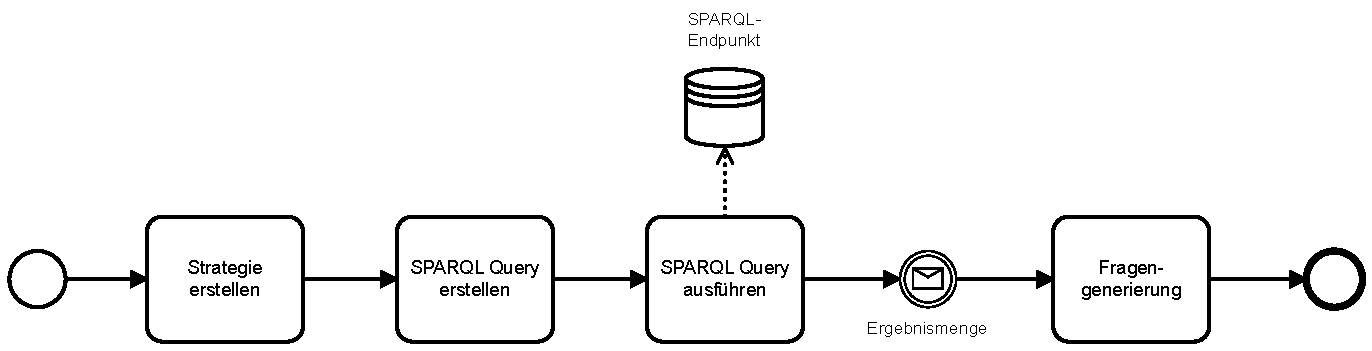
\includegraphics[width=\textwidth]{images/sparql-gen.pdf}
\caption{Die SPARQL-Abfrage im Ablauf.}
\label{img:sparql-question-generation}
\end{figure}

\begin{figure}
\centering
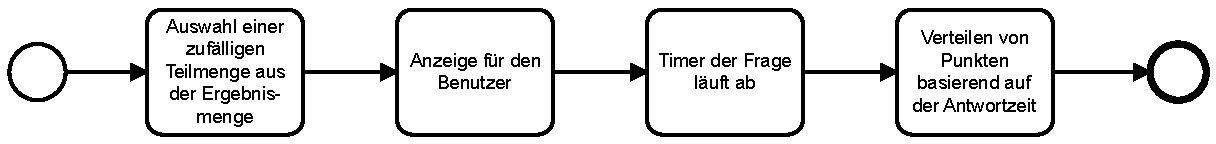
\includegraphics[width=\textwidth]{images/ausg-frage.pdf}
\caption{Ausgabe der Fragen an den Nutzer.}
\label{img:question-output-to-user}
\end{figure}

\chapter{Ausführung der Lösung}
%\todo{Die Ausführung der Lösung dient zur Erarbeitung von Konzepten zu den jeweiligen Ansätzen aus dem vorherigen Kapitel.}
\section{Lösung für Aufgabe A1.1}
\subsection{Untersuchen der bestehenden Queries}
\todo{Tatsächlichen Referrer zu 1.1.1 hinzufügen}
Wie in Abschnitt 1.1.1 bereits beschrieben wurde, gibt es bei dem existierenden Prototypen 2 Typen von Strategien, die zur Generierung von Fragen genutzt werden:
\begin{itemize}
\item die DEFINITION-Query (A defines B),
\item und die SUBJECT-Query (A is related to B in way C)
\end{itemize}
Die zwei vorhandenen Strategien generieren auf Basis dieser Queries Fragen.
Um die Verständlichkeit zu erhöhen, werde ich die erste Strategie umfangreicher erklären und umfangreicher auf bestimmte Operationen und Methoden eingehen.
\subsubsection{DEFINITION-Query}
Query:
\begin{lstlisting}
SELECT SAMPLE(replace(str(?def),str(?cl),"X","i") as ?def)
SAMPLE(str(?cl) as ?cl) 
SAMPLE(str(?a1l) as ?a1l)
SAMPLE(str(?a2l) as ?a2l)
SAMPLE(str(?a3l) as ?a3l)
# Gebe ?def, ?cl, ?a1l, ?a2l, ?a3l aus
(
?class a owl:Class.
# Sei ?class eine Klasse
?class rdfs:label ?cl.
# Sei ?cl der woertliche Bezeichner von ?class
FILTER(LANGMATCHES(LANG(?cl),"en"))
# Sei ?cl in englischer Sprache

?class skos:definition ?def.
# Sei ?def die Definition von ?class
FILTER(STRLEN(?def)>10&&STRLEN(?def)<600).
FILTER(LANGMATCHES(LANG(?def),"en"))
# Sei ?def in englischer Sprache und zwischen 10 und 600
  Zeichen lang

?class (!meta:subTopClass){1,2} ?a1,?a2,?a3.
# Seien ?a1, ?a2, ?a3 in direkter oder indirekter
  Nachbarschaft von ?class mit Pfadlaenge 1-2
# Pfad darf hierbei nicht ueber die meta:subTopClass fuehren

owl:Class ^a ?a1,?a2,?a3.FILTER(
?class!=?a1&&?class!=?a2&&?class!=?a3&&?a1<?a2&&?a2<?a3)
# Seien ?a1, ?a2, ?a3 Klassen
# Seien ?a1, ?a2, ?a3 paarweise verschieden und
  ungleich ?class

?a1 rdfs:label ?a1l.FILTER(LANGMATCHES(LANG(?a1l),"en"))
?a2 rdfs:label ?a2l.FILTER(LANGMATCHES(LANG(?a2l),"en"))
?a3 rdfs:label ?a3l.FILTER(LANGMATCHES(LANG(?a3l),"en"))
# Seien ?a1l, ?a2l, ?a3l die woertlichen Bezeichnungen von
  ?a1, ?a2, ?a3 in englischer Sprache
) GROUP BY ?class limit 1000

\end{lstlisting}

Die DEFINITION-Query dient als Ausführung der gleichnamigen Strategie der Generierung für Fragen, bei denen ein Parameter gegeben ist und ein anderer durch Antwortmöglichkeiten ausgewählt werden muss. 
Dabei ist im Speziellen hier eine Definition einer Klasse x vorgegeben, zu der diese Klasse x gesucht wird.
Die Ergebnismenge von ?class wird nun auf Klassen beschränkt.
Dadurch werden alle Attribute der Ontologie, die ein Element von owl:class sind, als potentielle Werte für ?class angesehen.
Einer zweiten Variable, ?cl, wird nun der Klarname der Klasse ?class in der gewünschten Sprache zugewiesen.

Hierbei ist ?class ist eine Kategorisierung, die eine Menge an Tripeln verbindet.
Dabei sieht sich ?class einem Primärschlüssel in SQL ähnlich: ein Identifier, der eindeutig und einzigartig ist.
Während die Klasse selbst neben einem Identifikationsschlüssel keine Informationen beinhaltet, finden sich diese Informationen in den Unterelementen wieder.
Dazu können beispielsweise Informationen wie Definitionen oder Ober- bzw. Unterklassen stecken.\\

\textit{Um das Beispiel \enquote{Skateboard} verständlich zu halten, bezieht es sich anstelle der SNIK-Ontologie auf Wikidata.
Wikidata ist eine Ontologie, die einen Großteil der Informationen der Wissenssammlung Wikipedia zusammenfasst.}\\\\

\enquote{Skateboard} ist hier als eigene Klasse mit dem Identifier \enquote{Q15783} gelistet. Sie besitzt unter anderem die Eigenschaft \enquote{label}, die mehrsprachig vorliegt.
Die Eigenschaft \enquote{label} beinhaltet den Klarnamen der ?class, also \enquote{Skateboard}, in verschiedenen Sprachen. 
Um nun die gewünschte Sprache auszuwählen, wird ein FILTER genutzt.
Dieser schließt hier alle Attribute der Eigenschaft label für ?class aus, die nicht in englischer Sprache sind.
Dieses Label wird in der Variable ?cl gespeichert.

Im nächsten Schritt wird auf ein weiteres Unterelement von ?class zugegriffen: der Definition.
Diese wird der Variable ?def zugewiesen und liegt erneut mehrsprachig vor.
Hier wird erneut auf FILTER zugegriffen, um nur englischsprachige Elemente anzuzeigen.
Weiterhin wird die Anzahl der Zeichen so beschränkt, dass nur Ergebnisse zwischen 10 und 600 Zeichen angezeigt werden.

Im nächsten Schritt werden nun die Distraktoren generiert.
Diese heißen im Beispiel ?a1,?a2 und ?a3 und sind ebenfalls Klassen, die jedoch nicht mit ?class (\enquote{Skateboard}) zusammenhängen dürfen.
Nun wird die Limitierung !subTopClass(1,2) gesetzt, die beschränkt, welche Entfernung die Elemente von ?class besitzen dürfen.
Diese Entfernung darf nicht über Oberelemente gemessen werden, sondern ausschließlich über Unterklassen. 

Im letzten Schritt werden die drei Variablen ?a1l, ?a2l und ?a3l mit den Labels von ?a1, ?a2, ?a3 versehen.
Nun werden die Variablen ?cl, ?a1l, ?a2l, ?a3l sowie ?def ausgegeben, wobei bei ?def noch jedes Vorkommen von ?cl durch X ersetzt wird.
Die Ausgabe der Query wäre nun:
\begin{table}
\begin{centering}
\begin{lstlisting}
?def: "Ein X, gelegentlich verdeutscht auch Rollbrett genannt,
ist ein Brett (Deck) mit zwei Achsen (Trucks) [...]"
?cl:  "Skateboard"
?a1l: "Pennyboard"
?a2l: "Rollschuhe"
?a3l: "Rollsportgeraete"
\end{lstlisting}
\end{centering}
\caption{Beispielausgabe der DEFINITION-Query in Datenform.}
\label{tab:sparqldefinitionexampledata}
\end{table}

Die eben generierte Fragestellung würde hier wie folgt aussehen:\\

\begin{table}
\begin{centering}
\begin{tabularx}{\textwidth}{XXX}
\toprule
%\textrm{Was wird hiervon definiert? \enquote{Ein X, gelegentlich verdeutscht auch Rollbrett genannt, ist ein Brett (Deck) mit zwei Achsen (Trucks) [...]}}\\
\multicolumn{2}{p{0.97\textwidth}}{Was wird hiervon definiert? \enquote{Ein X, gelegentlich verdeutscht auch Rollbrett genannt, ist ein Brett (Deck) mit zwei Achsen (Trucks) [...]}}\\
\midrule
Rollschuhe										&Rollsportgeräte\\
\textcolor{green}{Skateboard}			&Pennyboard\\
\bottomrule
\end{tabularx}
\end{centering}
\caption{Fragestellung der DEFINITION-Query.}
\label{tab:sparqldefinitionexample}
\end{table}

Hierbei ist \enquote{Skateboard} die richtige Antwortmöglichkeit. 

\begin{figure}
\centering
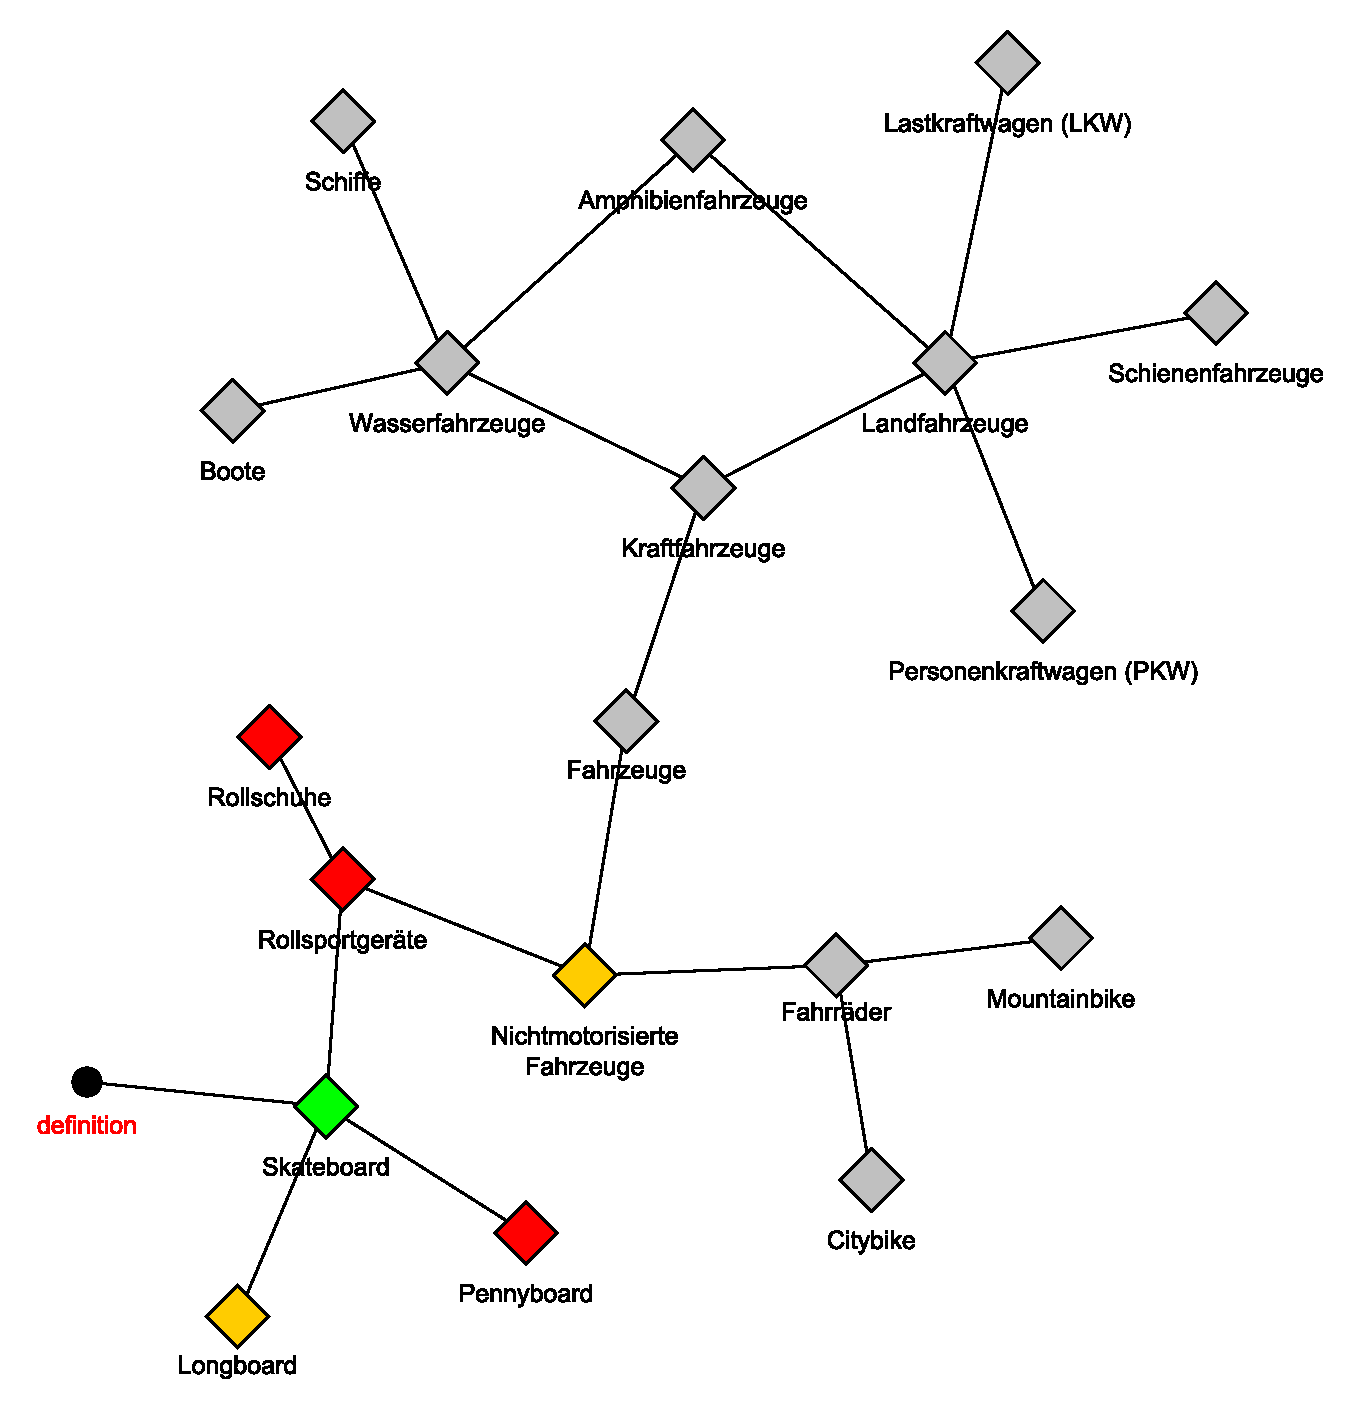
\includegraphics[width=\textwidth]{images/definition.pdf}
\caption{Fragengenerierung mithilfe der DEFINITION-Query.}
\label{img:definition-query-prototype}
\end{figure}


\subsubsection{CONTAINS-Query}
\begin{lstlisting}
SELECT DISTINCT ?p
?o
(min(?c1) as ?c1)
(min(?c2) as ?c2)
(min(?c3) as ?c3)
?c4
# Gebe ?p, ?o, ?c1, ?c2, ?c3, ?c4 aus
from <http://www.snik.eu/ontology/bb>
from <http://www.snik.eu/ontology/derived>
# Nutzung mehrerer Ontologien
{
 ?c1 meta:closeNeighbour ?c2,?c3,?c4. 
# Seien ?c2, ?c3, ?c4 direkte Nachbarn (Pfadlaenge 1) mit ?c1
 owl:Class ^a ?c1,?c2,?c3,?c4,?o.

 filter(?o!=?c1&&?o!=?c2&&?o!=?c3&&?o!=?c4).
 filter(?c1!=?c2&&?c1!=?c3&&?c1!=?c4&&?c1<?c2&&?c2<?c3&&?c3<?c4).
# Stelle sicher, dass die Antworten ungleich einander sind


 graph <http://www.snik.eu/ontology/bb>
 {?c1 ?p ?o.
# Sei ?c1 in Beziehung ?p mit ?o (richtige Antwort)
 FILTER(?p!=meta:isAssociatedWith).
# Entferne alle Beziehungen, die keine Beziehung verdeutlichen
 MINUS {?c2 ?p ?o} 
 MINUS {?c3 ?p ?o} 
 MINUS {?c4 ?p ?o} 
# Entferne alle Antwortmoeglichkeiten, die auch richtig waeren,
  da sie die selbe Beziehung wie die richtige Antwort zum Praedikat
  besitzen wuerden
 }
 
}
\end{lstlisting}

Die CONTAINS-Query wird als Strategie für Fragen genutzt, bei denen zwei Parameter gegeben sind und ein dritter zur Auswahl steht.
Hier ist dabei im Besonderen eine Klasse X und die Beziehung Y dieser Klasse X zu einer anderen Klasse Z gegeben, wobei hier Klasse Z gesucht wird.
Dabei verläuft die Fragengeneration ähnlich wie bei der DEFINITION-Query: Im ersten Schritt wird sichergestellt, dass ?c1, ?c2, ?c3 und ?c4 direkte Nachbarn miteinander sind.
Eine direkte Nachbarschaft im ontologischen Sinne wird dadurch kategorisiert, dass die Pfadlänge zwischen den einzelnen Elementen genau 1 beträgt.
Es kann dadurch keine Zwischenelemente geben, die zwischen den Klassen stehen.

Da nun die Generierung von vier untereinander benachbarten Antworten beendet ist, wird nun bei der ersten Antwort eine Beziehung zu einem Objekt hergestellt.
Diese Beziehung ?p zu Objekt ?o wird im nächsten Schritt auch zu den anderen 3 Antwortmöglichkeiten geprüft.
Besteht diese Beziehung dort ebenfalls, wird die potentielle Antwortmöglichkeit entfernt.
Stehen keine Antwortmöglichkeiten mehr zur Verfügung, wird das gesamte Anfangstripel übersprungen und die nächste Beziehung wird aufgebaut.

Am Ende werden die vier Antwortmöglichkeiten, das Objekt ?o und die Beziehung ?p ausgegeben. 


\chapter{Ergebnis}
\todo{
Im Ergebniskapitel soll beschrieben werden, inwiefern Sie Ihre in 1.2/1.3 aufgestellten Ziele bzw. Aufgaben erreicht habe oder auch weshalb sie (teilweise) nicht erreicht werden konnten.
So soll es möglich sein, dass ein Leser von der Arbeit lediglich die Einleitung und die Zusammenfassung liest und doch die Ergebnisse der Arbeit erfassen kann.
Dieses Kapitel kann auch in mehrere Unterkapitel aufgeteilt werden, wenn das sinnvoll ist!
}

\chapter{Diskussion und Ausblick \todo{1--2 Seiten}}
\todo{
In der Diskussion wird das Ergebnis der Arbeit noch einmal kritisch bewertet.
Dies umfasst auch neue Probleme, die erst während der Bearbeitung erkannt wurden.
Die Eignung für ein konkretes Forschungsprojekt sollte hier diskutiert werden.
In der Diskussion kann auch die Kritik des Autors an dem stehen, was er in der Literatur zu dem zu bearbeitenden Thema hier und da gelesen hat.
Außerdem soll ein Ausblick gegeben werden, welche weiteren Fragestellungen noch bearbeitet werden sollten.
}

\renewcommand{\bibpreamble}{
\todo{
Zentrale Literatur, die den untersuchten Artikeln zugrunde liegt, können Sie im bibtex-Format in die seminar.bib einfügen und dann im Text zitieren, wodurch diese automatisch in das Literaturverzeichnis übernommen werden.
Sie können auch weitere referierte Veröffentlichungen (wissenschaftliche Zeitschriften (auch elektronisch), Bücher) in die Erarbeitung einbeziehen zitieren.
Sie können dafür Literaturdatenbanken wie Pubmed oder Google Scholar durchsuchen und dort direkt als bibtex-Eintrag herunterladen.
Bitte beachten Sie, dass die \href{https://www.openoffice.org/bibliographic/bibtex-defs.html}{bibtex-Einträge vollständig sind}, z.B. sind das bei Büchern Autor, Editor, Title, Kapitel oder Seiten, Herausgeber und Jahr..
Weitere Informationen zum Thema der Literaturrecherche finden sich in den \href{http://www.imise.uni-leipzig.de/Lehre/MedInf/Abschlussarbeiten/Literaturrecherche.jsp}{Hinweisen zur Literaturrecherche}.
\paragraph{Beispielzitierungen}
\citet{his} beschreiben ein Verfahren zur X von Y auf Basis von Z.
Alternativ: X von Y lässt sich auf Basis von Z ermitteln~\citep{his}.
}
}

\bibliographystyle{dinat}
\bibliography{bell}

\end{document}